\documentclass[11pt]{article}
\title{Exact Fibonacci Corrections for Nonconsecutive Subset Sums Modulo Three}
\date{}
\author{SIGMA AI-assisted research synthesis}
\usepackage[T1]{fontenc}
\usepackage[utf8]{inputenc}
\usepackage[margin=1in]{geometry}
\usepackage{amsmath,amssymb,array,booktabs,longtable,pdflscape}
\usepackage{microtype}
\usepackage[hyphens]{url}
\usepackage{titlesec}
\usepackage{tikz}
\usetikzlibrary{fit}
\emergencystretch=2em
\raggedbottom
\linespread{1.07}
\usepackage{xcolor}
\definecolor{blue}{HTML}{24485E}
\titleformat{\section}{\Large\bfseries\sffamily\color{blue}}{\thesection}{0.8em}{}
\titleformat{\subsection}{\large\bfseries\sffamily}{\thesubsection}{0.7em}{}
\setlength{\parskip}{.6em}
\setlength{\parindent}{0pt}
\begin{document}
\maketitle

\begin{abstract}
How many subsets of an initial interval contain no consecutive integers and have sum divisible by three? We derive an exact formula for this count by separating the total number of admissible subsets from a smaller residue correction. A weighted subset recurrence and a cube-root filter reduce the problem to three explicit Fibonacci formulas, one for each index class modulo three. These identities yield a homogeneous order-eight recurrence with integer coefficients, eight sufficient initial values, and the exact value $a_{12}=128$. They also explain the limiting proportion: the total count grows on the Fibonacci scale, whereas the correction grows on the scale of a Fibonacci sequence indexed at one third of the original index.

An explicit exponential bound proves that $a_n/F_{n+2}$ tends to $1/3$. The argument establishes these conclusions symbolically, rather than inferring a recurrence from finitely many counts.
\end{abstract}
\section{Introduction}
For every integer $n\geq 0$, let $a_n$ count subsets $S\subseteq\{1,\ldots,n\}$ that contain no consecutive integers and satisfy $\sum_{i\in S}i\equiv 0\pmod 3$. The empty subset is included, so $a_0=1$. The question is to determine a constant-coefficient integer recurrence valid from a specified starting index, give sufficient initial values, compute $a_{12}$, and prove the limiting proportion relative to the total admissible count.

Write $F_0=0$, $F_1=1$, and $F_{k+2}=F_{k+1}+F_k$ for $k\geq 0$. The total number of subsets satisfying only the nonconsecutiveness condition is $F_{n+2}$. The central quantity is therefore the exact imbalance $c_n=3a_n-F_{n+2}$: determining this correction answers both the finite counting question and the asymptotic question without assuming that residues are equally frequent.

\section{Definitions and proof basis}
The analysis represents admissible subsets by their sum-weighted polynomial and partitions them according to whether the final position is selected. Evaluation at a primitive cube root of unity then isolates sums divisible by three. A complete induction across the three index phases establishes the weighted evaluations, including their initial triple; finite values serve as arithmetic checks rather than evidence for a universal pattern.

The exact correction formulas are combined with the Fibonacci recurrence through commuting polynomial shift operators. A complementary formal-power-series elimination supplies the rational generating function and checks the recurrence's starting index. Elementary Fibonacci bounds compare the correction with the total count and give an explicit all-index error estimate; the additional minimal-order assertion is separated from these conclusions because the bounded excerpts do not expose its complete coprimality calculation.

The bounded evidence index omitted 2809 saved research fragments across 7 sources. Claims that could depend on those fragments remain provisional; the full omission ledger is retained with the archived research record.
\section{Admissible subsets and the residue filter}
A weighted enumerator separates the Fibonacci count of nonconsecutive subsets from the correction imposed by divisibility of their sums by three. For an integer $n\geq 0$, call a subset $S\subseteq\{1,\ldots,n\}$ admissible if it contains no two consecutive integers, and let $a_n$ count the admissible subsets for which $3\mid\sum_{i\in S}i$. The ground set is empty when $n=0$; the empty subset is admissible and has sum zero, so it contributes to every $a_n$.

Write $F_0=0$, $F_1=1$, and $F_{k+2}=F_{k+1}+F_k$ for every integer $k\geq 0$. The main theorem, whose proof is developed below, is that the counts satisfy the integer-coefficient recurrence
$a_{n+8}=a_{n+7}+a_{n+6}+a_{n+5}-a_{n+4}-a_{n+3}+a_{n+2}-a_{n+1}-a_n$
for every integer $n\geq 0$, with sufficient initial values
$(a_0,a_1,a_2,a_3,a_4,a_5,a_6,a_7)=(1,1,1,2,3,5,8,12)$. In particular, $a_{12}=128$.

The theorem also gives the quantitative limiting statement
$0\leq \frac{a_n}{F_{n+2}}-\frac13\leq\frac23\varphi^{-2n/3}\qquad(n\geq 0),$
where $\varphi=(1+\sqrt5)/2$. Consequently, $a_n/F_{n+2}\to 1/3$ as $n\to\infty$. We first establish the exact counting identity from which the recurrence and the estimate will follow.

For an indeterminate $q$, define the polynomial
$P_n(q)=\sum_{S\text{ admissible}}q^{\sum_{i\in S}i},$
where the sum ranges over admissible subsets of $\{1,\ldots,n\}$. Each subset contributes one monomial, so the coefficient of a given power counts the subsets having that sum. The empty subset contributes the constant term, and the initial polynomials are $P_0(q)=1$ and $P_1(q)=1+q$.

For $n\geq 2$, partition the admissible subsets according to whether they contain $n$. Those omitting $n$ are precisely the admissible subsets of $\{1,\ldots,n-1\}$, and therefore contribute $P_{n-1}(q)$. Those containing $n$ must omit $n-1$; deleting $n$ leaves an admissible subset of $\{1,\ldots,n-2\}$. Conversely, adjoining $n$ to any admissible subset of this shorter interval creates no consecutive pair, because every remaining element is at most $n-2$.

The latter construction is reversible and increases the subset sum by exactly $n$, so its contribution is $q^nP_{n-2}(q)$. The two disjoint classes thus give the polynomial identity
$P_n(q)=P_{n-1}(q)+q^nP_{n-2}(q)\qquad(n\geq 2).$
At $q=1$, every admissible subset has weight one, and this identity becomes the Fibonacci recurrence with initial values $P_0(1)=1$ and $P_1(1)=2$. Hence $P_n(1)=F_{n+2}$ for every $n\geq 0$, establishing the total count used to normalize $a_n$.

To impose the divisibility condition, fix a primitive cube root of unity $\omega\in\mathbb C$, so that $\omega^3=1$, $\omega\neq 1$, and $1+\omega+\omega^2=0$. For every integer $s$, the expression $1+\omega^s+\omega^{2s}$ equals $3$ if $3\mid s$. If $s\equiv 1\pmod 3$, it equals $1+\omega+\omega^2=0$; if $s\equiv 2\pmod 3$, it equals $1+\omega^2+\omega=0$. Thus $(1+\omega^s+\omega^{2s})/3$ is exactly the indicator that $s$ is divisible by three.

Apply this indicator to the sum of each admissible subset and add over all such subsets. Since the sums are finite, the defining polynomial gives
$3a_n=P_n(1)+P_n(\omega)+P_n(\omega^2)=F_{n+2}+P_n(\omega)+P_n(\omega^2)\qquad(n\geq 0).$
This filter selects all subset sums divisible by three, rather than a single exponent of $P_n(q)$, and includes the zero sum of the empty subset.

Define the correction by $c_n=P_n(\omega)+P_n(\omega^2)$. The filter proves the exact decomposition $3a_n=F_{n+2}+c_n$, and therefore identifies $c_n$ with the integer $3a_n-F_{n+2}$. The counting problem is now reduced to determining the two primitive-root evaluations: the Fibonacci term accounts for the total number of admissible subsets, while their sum accounts exactly for the departure of $a_n$ from one third of that total.

\begin{figure}[!htbp]
\centering
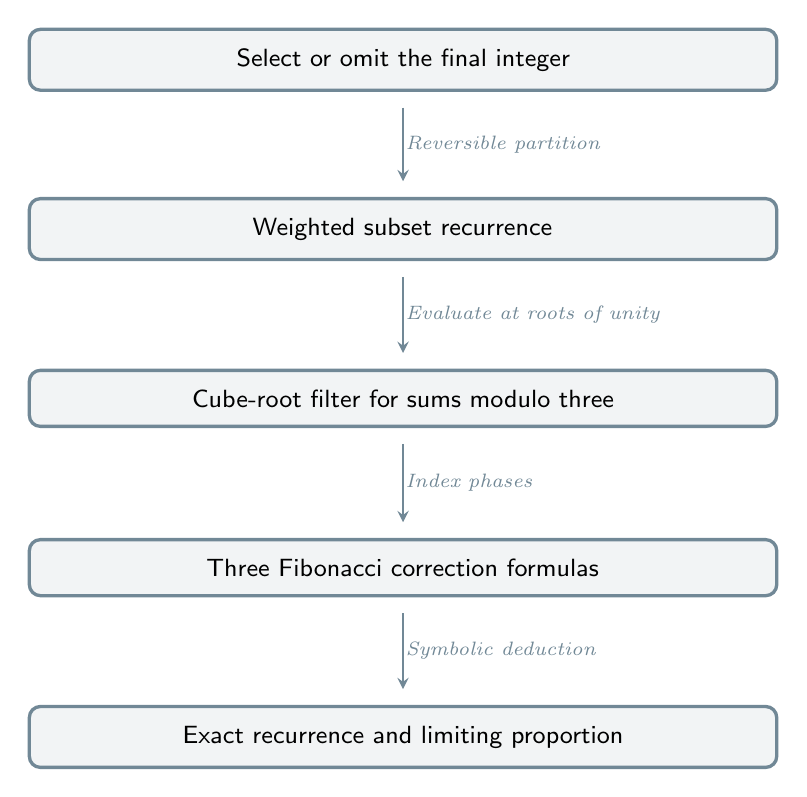
\begin{tikzpicture}[x=1cm,y=1cm,>=stealth,story node/.style={draw=blue!65,very thick,rounded corners=4pt,align=center,text width=9cm,font=\small\sffamily,fill=blue!6,inner sep=7pt}]
\node[story node] (partition) at (0,0.00) {Select or omit the final integer};
\node[story node] (polynomial) at (0,-2.15) {Weighted subset recurrence};
\node[story node] (filter) at (0,-4.30) {Cube-root filter for sums modulo three};
\node[story node] (correction) at (0,-6.45) {Three Fibonacci correction formulas};
\node[story node] (results) at (0,-8.60) {Exact recurrence and limiting proportion};
\draw[->,thick,blue!65,shorten <=2mm,shorten >=2mm] (partition) -- node[midway,right,font=\scriptsize\itshape,align=left,text width=3.8cm,fill=white,inner sep=1pt] {Reversible partition} (polynomial);
\draw[->,thick,blue!65,shorten <=2mm,shorten >=2mm] (polynomial) -- node[midway,right,font=\scriptsize\itshape,align=left,text width=3.8cm,fill=white,inner sep=1pt] {Evaluate at roots of unity} (filter);
\draw[->,thick,blue!65,shorten <=2mm,shorten >=2mm] (filter) -- node[midway,right,font=\scriptsize\itshape,align=left,text width=3.8cm,fill=white,inner sep=1pt] {Index phases} (correction);
\draw[->,thick,blue!65,shorten <=2mm,shorten >=2mm] (correction) -- node[midway,right,font=\scriptsize\itshape,align=left,text width=3.8cm,fill=white,inner sep=1pt] {Symbolic deduction} (results);
\end{tikzpicture}
\caption{Proof map for the exact count. The select-or-omit partition gives the weighted recurrence; the cube-root filter isolates sums divisible by three; the three index phases yield Fibonacci correction formulas, from which the order-eight recurrence and limiting proportion follow. The diagram summarizes the proof dependencies rather than replacing them.}
\par\smallskip{\scriptsize Source-linked claims: C1, C2, C3, C4, C5, C9; evidence links appear in the claim notes.}
\end{figure}
\section{Three-phase Fibonacci formulas}
The primitive-root contributions admit exact Fibonacci formulas on each index class modulo three, turning the residue filter into an explicit correction to the total count. Let $\omega$ be a primitive complex cube root of unity, so $\omega^3=1$ and $1+\omega+\omega^2=0$, and put $p_n=P_n(\omega)$ for the weighted subset enumerator defined above. Its recurrence becomes $p_n=p_{n-1}+\omega^n p_{n-2}$ for every integer $n\geq 2$; the multiplier therefore passes successively through $1$, $\omega$, and $\omega^2$ as the index advances through a complete triple.

We claim that, for every integer $m\geq 0$,
$P_{3m}(\omega)=F_{m+1}+\omega F_m,\qquad P_{3m+1}(\omega)=(1+\omega)F_{m+1},\qquad P_{3m+2}(\omega)=F_m.$
We prove these identities simultaneously by induction on $m$, advancing all three phases at each step. The initial polynomials give $p_0=1$, $p_1=1+\omega$, and $p_2=1+\omega+\omega^2=0$. These are precisely the claimed values at $m=0$, since $F_0=0$ and $F_1=F_2=1$.

Suppose the three identities hold for some integer $m\geq 0$. At the first index of the next triple, the multiplier is $\omega^{3m+3}=1$, so
$p_{3m+3}=p_{3m+2}+p_{3m+1}=F_m+(1+\omega)F_{m+1}=F_{m+2}+\omega F_{m+1}.$
The last equality uses $F_{m+2}=F_{m+1}+F_m$, and establishes the first identity with $m$ replaced by $m+1$.

At the next index, the multiplier is $\omega^{3m+4}=\omega$. Substituting the value just obtained and the induction hypothesis yields
$p_{3m+4}=p_{3m+3}+\omega p_{3m+2}=F_{m+2}+\omega(F_{m+1}+F_m)=(1+\omega)F_{m+2}.$
Thus the second identity also advances, again by the Fibonacci recurrence.

The final phase uses $\omega^{3m+5}=\omega^2$, and here the cube-root cancellation is decisive:
$p_{3m+5}=p_{3m+4}+\omega^2p_{3m+3}=(1+\omega+\omega^2)F_{m+2}+\omega^3F_{m+1}=F_{m+1}.$
This is the third identity for $m+1$. The base triple and these three successive deductions establish the formulas at every nonnegative index.

The same proof applies to the other primitive root, $\omega^2$: replacing $\omega$ by $\omega^2$ gives $P_{3m}(\omega^2)=F_{m+1}+\omega^2F_m$, $P_{3m+1}(\omega^2)=(1+\omega^2)F_{m+1}$, and $P_{3m+2}(\omega^2)=F_m$. Define the integer correction by $c_n=3a_n-F_{n+2}$. The residue-filter identity and $P_n(1)=F_{n+2}$ identify it as $c_n=P_n(\omega)+P_n(\omega^2)$, so adding the paired formulas and using $\omega+\omega^2=-1$ gives
$c_{3m}=2F_{m+1}-F_m,\qquad c_{3m+1}=F_{m+1},\qquad c_{3m+2}=2F_m\qquad(m\geq 0).$

These formulas also give a constant-coefficient recurrence for the correction itself. For each fixed $r\in\{0,1,2\}$, let $b_m=c_{3m+r}$ for integers $m\geq 0$; the displayed expressions make $b_m$ a fixed linear combination of $F_m$ and $F_{m+1}$. Since both Fibonacci sequences satisfy the same recurrence in $m$, their linear combination satisfies $b_{m+2}=b_{m+1}+b_m$ for every $m\geq 0$. Writing each nonnegative integer uniquely as $n=3m+r$ therefore yields
$c_{n+6}=c_{n+3}+c_n\qquad(n\geq 0).$

The exact decomposition $3a_n=F_{n+2}+c_n$ thus separates two Fibonacci structures with different index increments: the total count follows the ordinary Fibonacci recurrence, while the residue correction follows it along each subsequence of indices spaced three apart. The correction is consequently not an unspecified remainder in the counting formula, but an explicitly determined sequence with its own recurrence.

\section{The integer recurrence and exact counts}
The exact Fibonacci decomposition yields a single constant-coefficient recurrence for the counting sequence, with integer coefficients and validity from the first nonnegative index. Write $f_n=F_{n+2}$ and retain the correction $c_n=3a_n-f_n$, so that $3a_n=f_n+c_n$. The identities established above give $f_{n+2}=f_{n+1}+f_n$ and $c_{n+6}=c_{n+3}+c_n$ for every integer $n\geq 0$; these two recurrences supply the factors of the required recurrence.

For a sequence $u=(u_n)_{n\geq 0}$, define the forward-shift operator $E$ by $(Eu)_n=u_{n+1}$. Put $L(E)=E^2-E-1$ and $H(E)=E^6-E^3-1$. To say that such an operator annihilates a sequence means that its application gives the zero sequence, so the component identities are precisely $L(E)f=0$ and $H(E)c=0$. Since both operators are polynomials in the same forward shift, they commute, and hence
$L(E)H(E)(f+c)=H(E)L(E)f+L(E)H(E)c=0.$
Thus their product annihilates $3a$ and, by linearity, also $a$.

Expanding the product gives
$(E^2-E-1)(E^6-E^3-1)=E^8-E^7-E^6-E^5+E^4+E^3-E^2+E+1.$
Consequently, for every integer $n\geq 0$, the desired counts satisfy
$a_{n+8}=a_{n+7}+a_{n+6}+a_{n+5}-a_{n+4}-a_{n+3}+a_{n+2}-a_{n+1}-a_n.$
The index range is preserved in this argument: both component identities hold at every nonnegative index, and composing forward shifts uses only later indices. In particular, no negative-index extension or eventual-recurrence qualification is needed.

The exact correction formulas give $(c_0,\ldots,c_7)=(2,1,0,1,1,2,3,2)$, while the corresponding Fibonacci values are $(F_2,\ldots,F_9)=(1,2,3,5,8,13,21,34)$. Applying $a_n=(F_{n+2}+c_n)/3$ gives the eight starting counts:
$\begin{array}{c|rrrrrrrr} n&0&1&2&3&4&5&6&7\\ \hline a_n&1&1&1&2&3&5&8&12 \end{array}$
Because the coefficient of $a_{n+8}$ is one, the recurrence determines each next term uniquely from the preceding eight terms. These initial values are therefore sufficient to specify the entire counting sequence.

At its first application, the recurrence gives
$a_8=12+8+5-3-2+1-1-1=19.$
This checks the signs and the starting index by exact substitution; the universal validity of the recurrence comes from the annihilator argument, not from this finite calculation.

For the requested count, the correction formula at $12=3\cdot 4$ gives $c_{12}=2F_5-F_4=10-3=7$. Since $F_{14}=377$, the exact decomposition yields
$a_{12}=\frac{F_{14}+c_{12}}{3}=\frac{377+7}{3}=128.$
The decomposition therefore supplies both an exact evaluation and a finite integer recurrence determining all later counts, rather than merely a pattern among the initial values.

\section{The rational generating function and the order question}
The rational generating function explains why the recurrence combines a Fibonacci factor with a factor involving powers divisible by three. This explanation comes directly from the weighted counting recurrence, rather than from matching a finite list of counts. It also separates two logically distinct questions: whether an order-eight recurrence holds from its first possible instance, and whether any recurrence of smaller order can hold, even eventually.

Fix a primitive cube root $q$, so that $q^3=1$ and $1+q+q^2=0$, and work in the formal power-series ring $\mathbb{Q}(q)[[x]]$. Recall that $P_n(q)$ is the weighted enumerator of admissible subsets, with $P_0(q)=1$, $P_1(q)=1+q$, and $P_n(q)=P_{n-1}(q)+q^nP_{n-2}(q)$ for $n\geq2$. Define $G(x)=\sum_{n\geq0}P_n(q)x^n$. Summing the recurrence over $n\geq2$ gives $G(x)-1-(1+q)x=x(G(x)-1)+q^2x^2G(qx)$, and therefore
$(1-x)G(x)=1+qx+q^2x^2G(qx).$
The initial contributions are explicit, so no negative-index convention is needed.

Replacing $x$ by $qx$ and then by $q^2x$ produces the other two equations:
$(1-qx)G(qx)=1+q^2x+qx^2G(q^2x)$
and
$(1-q^2x)G(q^2x)=1+x+x^2G(x).$
Thus the three substitutions close: after the third equation, the unknown series is again $G(x)$. Successive substitution into the first equation, followed by multiplication by $(1-qx)(1-q^2x)$, yields
$\bigl((1-x)(1-qx)(1-q^2x)-x^6\bigr)G(x)=(1+qx)(1-qx)(1-q^2x)+q^2x^2(1+q^2x)(1-q^2x)+x^4(1+x).$

The numerator in this elimination is essential, since it retains the initial terms as well as the recurrence structure. Its three contributions expand respectively to $1-q^2x-q^2x^2+qx^3$, $q^2x^2-x^4$, and $x^4+x^5$; the terms of degrees two and four cancel. Since $(1-x)(1-qx)(1-q^2x)=1-x^3$, the resulting identity is
$G(x)=\frac{1-q^2x+qx^3+x^5}{1-x^3-x^6}.$
Every denominator used has constant term one and is therefore invertible in the formal power-series ring; analytic convergence plays no role.

Let $b_n=P_n(q)+P_n(q^2)$ and $B(x)=\sum_{n\geq0}b_nx^n$. Adding the preceding rational identity to its counterpart with $q$ replaced by $q^2$, and using $q+q^2=-1$, gives
$B(x)=\frac{2+x-x^3+2x^5}{1-x^3-x^6}.$
For the total count, the Fibonacci recurrence and its first two terms give $\sum_{n\geq0}F_{n+2}x^n=(1+x)/(1-x-x^2)$. Consequently, the residue-filter identity $3a_n=F_{n+2}+b_n$ implies
$3A(x)=\frac{1+x}{1-x-x^2}+\frac{2+x-x^3+2x^5}{1-x^3-x^6},\qquad A(x)=\sum_{n\geq0}a_nx^n.$

Combining these fractions proves the formal identity
$A(x)=\frac{N(x)}{D(x)}=\frac{1-x^2-x^3+x^5-x^6-x^7}{(1-x-x^2)(1-x^3-x^6)}.$
The two denominator factors thus have separate origins: $1-x-x^2$ comes from the unrestricted admissible count, whereas $1-x^3-x^6$ comes from the primitive-root contribution. Expanding their product gives $D(x)=1-x-x^2-x^3+x^4+x^5-x^6+x^7+x^8$. Because $\deg N=7$, the identity $D(x)A(x)=N(x)$ implies $[x^{n+8}]D(x)A(x)=0$ for every $n\geq0$, which is precisely
$a_{n+8}-a_{n+7}-a_{n+6}-a_{n+5}+a_{n+4}+a_{n+3}-a_{n+2}+a_{n+1}+a_n=0.$
In particular, the numerator establishes the starting index, not merely eventual validity.

Minimality requires a further statement that coefficient extraction alone does not supply: the numerator and denominator must be coprime over $\mathbb{Q}$. To isolate its role, suppose an eventual homogeneous constant-coefficient recurrence of order $d$ has the normalized form $a_m=c_1a_{m-1}+\cdots+c_da_{m-d}$, with coefficients in $\mathbb{Q}$. For $R(x)=1-c_1x-\cdots-c_dx^d$, that recurrence makes $R(x)A(x)$ a polynomial, because all sufficiently high coefficients vanish. Substituting $A=N/D$ then gives $D\mid RN$; if $\gcd(N,D)=1$, it follows that $D\mid R$, hence $d\geq\deg D=8$.

The additional assertion that the displayed fraction is reduced is kept separate here from the established generating-function identity; the exact outstanding condition for the minimal-order conclusion is $\gcd(N,D)=1$ in $\mathbb{Q}[x]$. No cancellation analysis is needed for the recurrence already proved, since multiplying by the displayed denominator remains valid whether or not cancellation is possible. The generating function therefore identifies the structural source of the order-eight recurrence and certifies its full starting range, while making explicit the additional algebraic condition that would turn existence into minimality.

\section{Exponential decay of the relative correction}
The exact Fibonacci correction yields a quantitative limiting proportion: the excess over one third is nonnegative for every index and decays exponentially after normalization by the total count. Recall that $c_n=3a_n-F_{n+2}$ for every integer $n\geq 0$. We compare an upper bound for this correction, involving Fibonacci numbers indexed near $n/3$, with a lower bound for the total $F_{n+2}$.

For every integer $m\geq 0$, the established formulas are $c_{3m}=2F_{m+1}-F_m$, $c_{3m+1}=F_{m+1}$, and $c_{3m+2}=2F_m$. Since $0\leq F_m\leq F_{m+1}$, each expression is nonnegative and at most $2F_{m+1}$; in particular, the subtraction in the first formula cannot produce a negative correction. Writing an arbitrary index as $n=3m+r$, where $r\in\{0,1,2\}$, therefore gives the uniform estimate
$0\leq c_n\leq 2F_{\lfloor n/3\rfloor+1}\qquad(n\geq 0).$
This includes $c_0=2$ and the vanishing correction $c_2=0$.

Let $\varphi=(1+\sqrt{5})/2$, so that $\varphi>1$ and $\varphi^2=\varphi+1$. The elementary upper bound needed here is $F_{k+1}\leq\varphi^k$ for every integer $k\geq 0$. Its two base cases are $F_1=1=\varphi^0$ and $F_2=1\leq\varphi$. If it holds at two consecutive indices $k$ and $k+1$, then the Fibonacci recurrence gives $F_{k+3}=F_{k+2}+F_{k+1}\leq\varphi^{k+1}+\varphi^k=\varphi^{k+2}$, completing the induction.

A separate induction gives $F_{n+2}\geq\varphi^n$ for every integer $n\geq 0$. Here the base cases are $F_2=1=\varphi^0$ and $F_3=2\geq\varphi$. Given the bound at indices $n$ and $n+1$, the recurrence yields $F_{n+4}=F_{n+3}+F_{n+2}\geq\varphi^{n+1}+\varphi^n=\varphi^{n+2}$. Consequently, the correction and the total satisfy $c_n\leq 2\varphi^{\lfloor n/3\rfloor}$ and $F_{n+2}\geq\varphi^n$, respectively.

Because $F_{n+2}>0$, division of the exact identity $3a_n=F_{n+2}+c_n$ now gives
$0\leq\frac{a_n}{F_{n+2}}-\frac13=\frac{c_n}{3F_{n+2}}\leq\frac23\varphi^{\lfloor n/3\rfloor-n}\leq\frac23\varphi^{-2n/3}\qquad(n\geq 0).$
The last inequality uses $\lfloor n/3\rfloor\leq n/3$ and $\varphi>1$. At $n=0$, both the normalized excess and the final upper bound equal $2/3$, so the estimate also covers the empty ground set.

The upper bound tends to zero as $n\to\infty$, proving $\lim_{n\to\infty}a_n/F_{n+2}=1/3$. Thus the divisible-by-three proportion converges to one third while remaining at least one third at every finite index. The mechanism is the separation of Fibonacci scales: the correction is controlled at the shorter index $\lfloor n/3\rfloor+1$, whereas the total is indexed by $n+2$. The limiting proportion therefore follows from the exact correction identities and explicit inequalities, rather than from an assumed equidistribution of subset sums.

\section{Verification status and limitations}
\begin{itemize}
\item The supported proof is an ordinary symbolic mathematical derivation, not a machine-checked or independently externally verified certificate; finite arithmetic checks are not presented as a universal proof.
\item The bounded selection does not expose every calculation in the reported minimal-order argument. Minimality is therefore excluded from the main theorem and remains a separate reconstruction obligation.
\item The contribution concerns the stated nonconsecutiveness restriction and divisibility by three. No extension to other moduli, other spacing restrictions, or literature novelty is asserted.
\end{itemize}
\section{Open obligations}
\begin{itemize}
\item To include minimality as an established theorem, recover the full coprimality calculation for $N(x)=1-x^2-x^3+x^5-x^6-x^7$ and $D(x)=(1-x-x^2)(1-x^3-x^6)$ over $\mathbb{Q}$. The reconstruction must include the reported modular remainders, the integral-factor lifting argument, and the treatment of degree loss under reduction.
\item If minimality is retained, give the complete argument that a reduced generating-function denominator divides the denominator associated with any eventual homogeneous constant-coefficient recurrence. This is additional to, and unnecessary for, the requested recurrence, exact value, and limit.
\end{itemize}
\section{Conclusion}
The counting sequence is determined by the order-eight integer recurrence in C5 and the eight initial values in C6. The exact requested count is $a_{12}=128$.

The essential structural result is the explicit correction $3a_n-F_{n+2}$, whose three index phases are Fibonacci expressions on a shorter scale. Its relative contribution satisfies $0\leq a_n/F_{n+2}-1/3\leq (2/3)\varphi^{-2n/3}$, proving the limiting proportion $1/3$ without computational pattern matching.

The rational generating function explains the recurrence factors. Its reported reducedness and the resulting minimal-order assertion require fuller proof detail than the bounded selection supplies, so they do not strengthen the main theorem in this plan.

\section*{Claim and source notes}
These notes identify the saved evidence for claims used in the article. The complete claim register and reasoning are retained in the paper record.
\begin{sloppypar}
\small
\begin{description}
\item[C1] For integers $n\geq 0$, define $P_n(q)=\sum_S q^{\sum_{i\in S}i}$ over subsets $S\subseteq\{1,\ldots,n\}$ with no consecutive elements. Then $P_0(q)=1$, $P_1(q)=1+q$, and $P_n(q)=P_{n-1}(q)+q^nP_{n-2}(q)$ for every $n\geq 2$. In particular, $P_n(1)=F_{n+2}$. \textit{Status: }established.
\textit{Evidence: }[Project overview], [Research session 1, artifact 5], [Research session 1, artifact 6]
\item[C2] If $\omega^3=1$ and $\omega\ne 1$, then $3a_n=F_{n+2}+P_n(\omega)+P_n(\omega^2)$ for every integer $n\geq 0$. \textit{Status: }established.
\textit{Evidence: }[Research session 1, artifact 1], [Research session 1, artifact 6]
\item[C3] For every integer $m\geq 0$, the primitive-cube-root evaluations are $P_{3m}(\omega)=F_{m+1}+\omega F_m$, $P_{3m+1}(\omega)=(1+\omega)F_{m+1}$, and $P_{3m+2}(\omega)=F_m$. \textit{Status: }established.
\textit{Evidence: }[Research session 1, artifact 5], [Research session 1, artifact 2]
\item[C4] The correction $c_n=3a_n-F_{n+2}$ has the exact formulas $c_{3m}=2F_{m+1}-F_m$, $c_{3m+1}=F_{m+1}$, and $c_{3m+2}=2F_m$ for every integer $m\geq 0$. Consequently, $c_{n+6}=c_{n+3}+c_n$ for every integer $n\geq 0$. \textit{Status: }established.
\textit{Evidence: }[Research session 1, artifact 2], [Research session 1, artifact 5]
\item[C5] For every integer $n\geq 0$, the counts satisfy $a_{n+8}=a_{n+7}+a_{n+6}+a_{n+5}-a_{n+4}-a_{n+3}+a_{n+2}-a_{n+1}-a_n$. \textit{Status: }established.
\textit{Evidence: }[Research session 1, artifact 1], [Research session 1, artifact 5], [Research session 1, artifact 6]
\item[C6] Sufficient initial values are $(a_0,a_1,a_2,a_3,a_4,a_5,a_6,a_7)=(1,1,1,2,3,5,8,12)$, and the requested exact value is $a_{12}=128$. The first recurrence application gives $a_8=19$. \textit{Status: }established.
\textit{Evidence: }[Research session 1, artifact 1], [Research session 1, artifact 6], [Research session 1, artifact 5]
\item[C7] As a formal power series, $A(x)=\sum_{n\geq 0}a_nx^n$ satisfies $A(x)=(1-x^2-x^3+x^5-x^6-x^7)/[(1-x-x^2)(1-x^3-x^6)]$. \textit{Status: }established.
\textit{Evidence: }[Research session 1, artifact 4], [Research session 1, artifact 6]
\item[C8] The rational expression in C7 is reported to be reduced, which would make eight the minimal order over $\mathbb{Q}$ among homogeneous constant-coefficient recurrences for $a_n$, even when a recurrence is required only eventually. \textit{Status: }unresolved.
\textit{Evidence: }[Research session 1, artifact 4], [Research session 1, artifact 6]
\item[C9] With $\varphi=(1+\sqrt{5})/2$, every integer $n\geq 0$ satisfies $0\leq a_n/F_{n+2}-1/3\leq (2/3)\varphi^{-2n/3}$. In particular, $a_n/F_{n+2}\to 1/3$. \textit{Status: }established.
\textit{Evidence: }[Research session 1, artifact 5], [Research session 1, artifact 6]
\item[C10] The supplied mathematical derivations are exact symbolic arguments with finite arithmetic checks, but they have not been independently formally verified; the available evidence is a bounded selection rather than a complete inspection of every saved proof. \textit{Status: }limitation.
\textit{Evidence: }[Research session 1, artifact 5], [Research session 1, artifact 6], [Research session 1]
\end{description}
\end{sloppypar}
\section*{Paper writing source material used}
These sources informed manuscript organization and writing methods, not the scientific evidence or findings.
\begin{itemize}
\item Keith Conrad \textemdash{} Advice on Mathematical Writing (full text) (discipline): \url{https://kconrad.math.uconn.edu/blurbs/proofs/writingtips.pdf}
\item PLOS ONE \textemdash{} Manuscript and Reporting Guidelines (general): \url{https://journals.plos.org/plosone/s/submission-guidelines}
\item EASE \textemdash{} Guidelines for Authors of Scientific Articles (full text) (general): \url{https://pmc.ncbi.nlm.nih.gov/articles/PMC4130677/}
\end{itemize}
\section*{Authorship note}
AI-assisted synthesis from saved research; not independently peer reviewed.
\end{document}
